\documentclass{beamer}
%
% Choose how your presentation looks.
%
% For more themes, color themes and font themes, see:
% http://deic.uab.es/~iblanes/beamer_gallery/index_by_theme.html
%
\mode<presentation>
{
  \usetheme{Madrid}      % or try Darmstadt, Madrid, Warsaw, ...
  \usecolortheme{crane} % or try albatross, beaver, crane, ...
  \usefonttheme{default}  % or try serif, structurebold, ...
  \setbeamertemplate{navigation symbols}{}
  \setbeamertemplate{caption}[numbered]
  
} 

\usepackage[english]{babel}
\usepackage[utf8x]{inputenc}
\usepackage{courier}
\usepackage{dsfont}
\usepackage{verbatim} 
\usepackage{tikz}
\usepackage{caption}
\usepackage{multirow}
\usepackage{amsmath}
\usepackage{venndiagram}
\usepackage{xcolor}
\usepackage[shortlabels]{enumitem}
\usepackage{listings}
\usepackage{hyperref}
\hypersetup{
    colorlinks=true,
    linkcolor=blue,
    filecolor=magenta,      
    urlcolor=cyan,
}
\usepackage{subfigure}

\newcommand{\code}[1]{\texttt{#1}}
\graphicspath{{img/}}

\DeclareMathOperator*{\argmax}{arg\!\max}
\DeclareMathOperator*{\argmin}{arg\!\min}
\newcommand{\vp}{\vspace{2mm}}
\newcommand{\xt}{\texttt}

\usetikzlibrary{shapes,decorations,arrows,calc,arrows.meta,fit,positioning}
\tikzset{
    -Latex,auto,node distance =1 cm and 1 cm,semithick,
    state/.style ={ellipse, draw, minimum width = 0.7 cm},
    point/.style = {circle, draw, inner sep=0.04cm,fill,node contents={}},
    bidirected/.style={Latex-Latex,dashed},
    el/.style = {inner sep=2pt, align=left, sloped}
}

\usepackage{color}
\providecommand{\pb}[1]{\textcolor{red}{#1}}
\providecommand{\cn}[1]{\textcolor{blue}{#1}}

\usepackage{listings}
\lstdefinestyle{rstyle}{
	language=R,
    %stringstyle=\color{green},
    %otherkeywords={0,1,2,3,4,5,6,7,8,9},
    %morekeywords={TRUE,FALSE},
    %deletekeywords={data,frame,length,as,character}
    %keywordstyle=\color{blue},
    %commentstyle=\color{cyan},
}

\setitemize{label=\usebeamerfont*{itemize item}%
  \usebeamercolor[fg]{itemize item}
  \usebeamertemplate{itemize item}}

\newcommand{\Mypm}{\mathbin{\tikz [x=1.4ex,y=1.4ex,line width=.1ex] \draw (0.0,0) -- (1.0,0) (0.5,0.08) -- (0.5,0.92) (0.0,0.5) -- (1.0,0.5);}}%

\title[Public Defense]{What You See is What You Get:}
\subtitle{A Closer Look at Bias in the Visual World Paradigm}
\author{Collin Nolte}
\date{March 8, 2023}

\begin{document}

\begin{frame}
  \titlepage
\end{frame}


\begin{frame}
\begin{center}
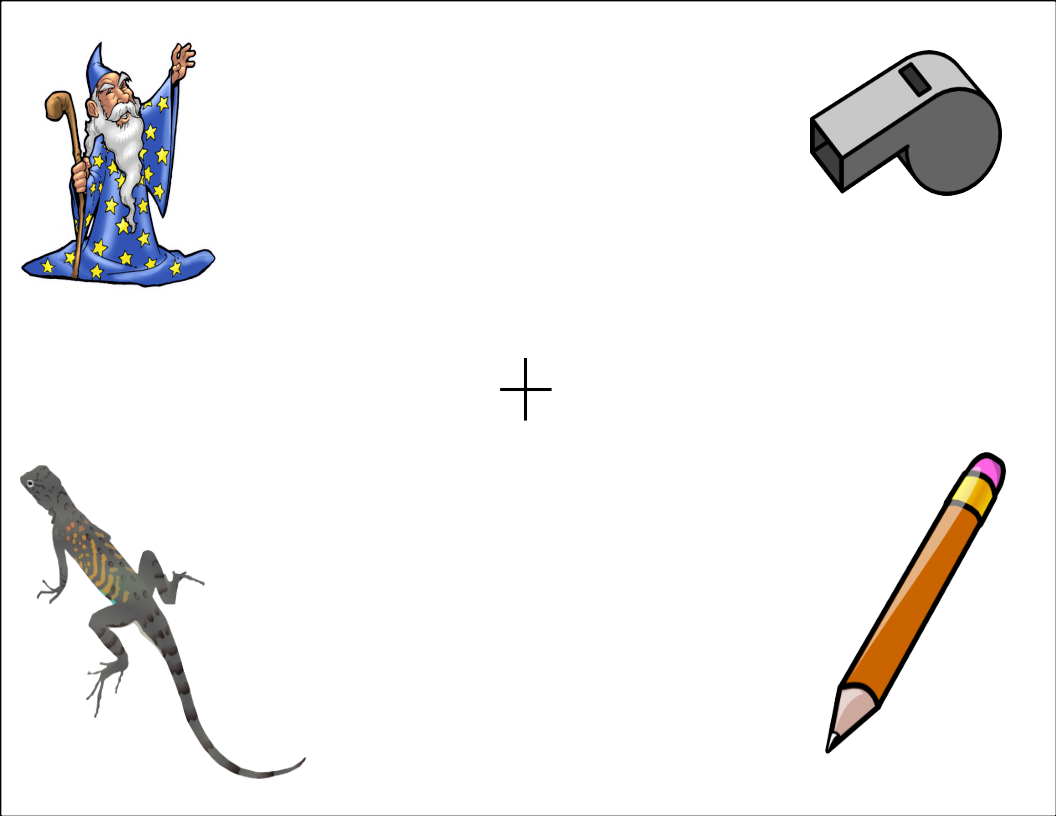
\includegraphics[scale=0.35]{img/wizard_lizard_whistle_pencil.png}
\end{center}
\end{frame}

%\begin{frame}{img (delete slide)}
%here just have a picture of a vwp trial w/o context. While the picture is up, ask some questions: 
%
%\begin{itemize}
%\item what are some images on screen? any obvious relations? (rhymes, begin same)
%\item If I told you to look at the wizard, how might i be able to tell when you understand exactly what I meant? (hopefully they answer eyes)
%\item what are some things i should be aware of when considering eyes (scanning, back and forth, etc)
%\end{itemize}
%\end{frame}

\begin{frame}{Outline}\Large
What is this talk going to be about?

\begin{itemize}
	\item Cognition/Activation 
	\item Eyetracking and the VWP
	\item Methodology and Bias
	\item Future Directions
\end{itemize}

\end{frame}

% language and cognition
\begin{frame}{Language and Cognition}\large
The field is itself exceptionally broad, ranging from sentence processing, priming, reading, and word formation:

\begin{center}
``trink" $\Rightarrow$ ``trank" or ``trinked"? \vp
\end{center}

Particularly troublesome when we commit too early:

\begin{center}
``The horse raced past the barn fell"  \vp
\end{center}

Often can not be observed directly  \vp

Limit focus to single word recognition \cn{start by introducing cohort model as an idea}



%This is such a seriously huge topic ranging from word recognition to sentence comprehension \\
%This also extends to thinks like reading \\
%Here, we are going to limit our consideration to single word recogntion \\
%It all starts with an audio signal that is interpreted by our brains in real time
\end{frame}

% cohort illustration

\begin{frame}
\begin{center}
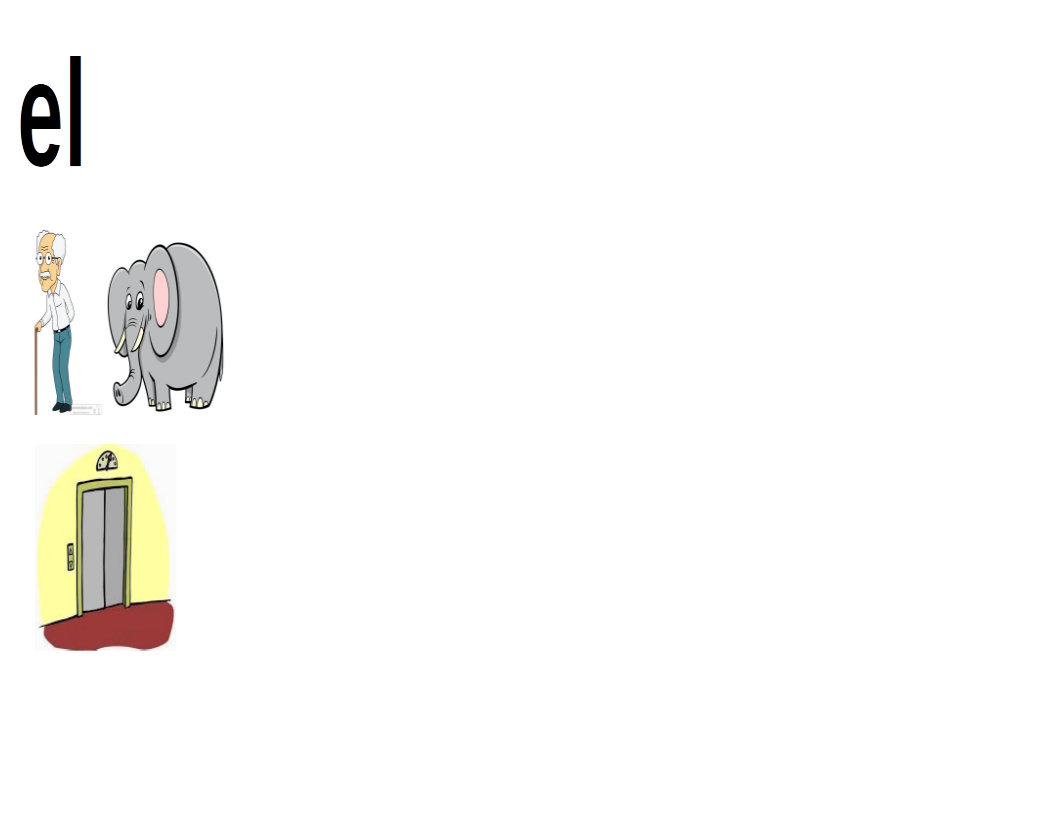
\includegraphics[scale=0.3]{img/ele_1.png}
\end{center}
\end{frame}

\begin{frame}
\begin{center}
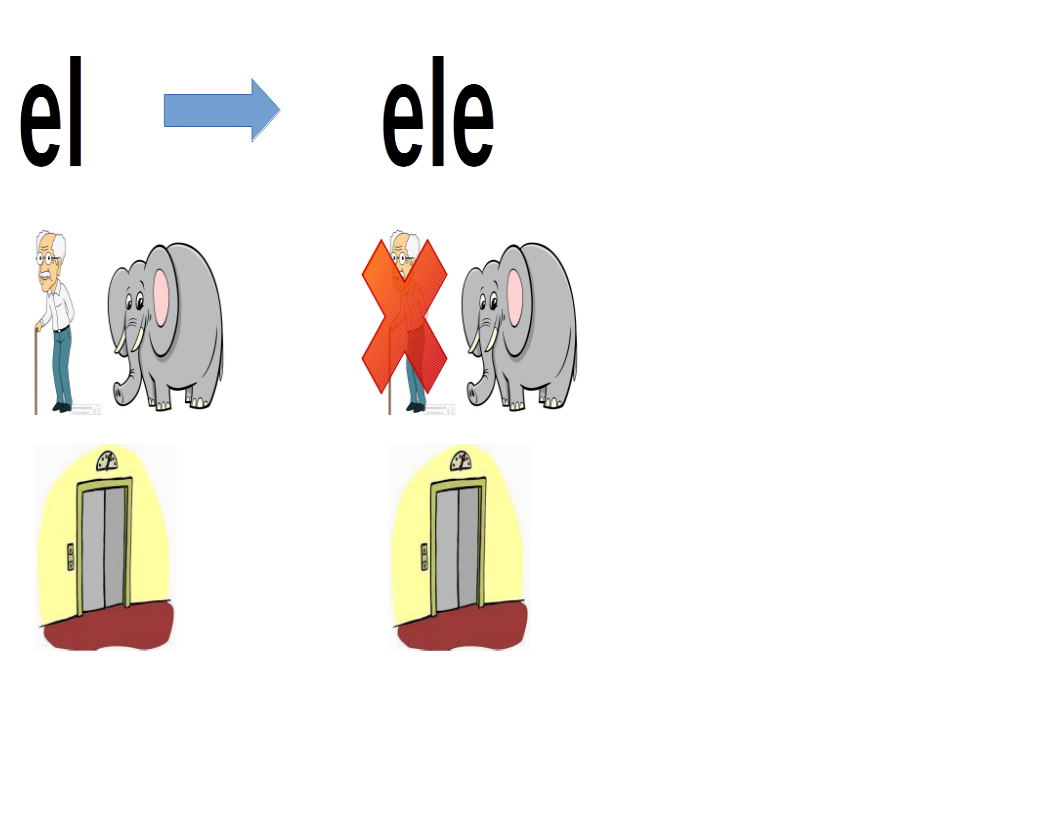
\includegraphics[scale=0.3]{img/ele_2.png}
\end{center}
\end{frame}

\begin{frame}
\begin{center}
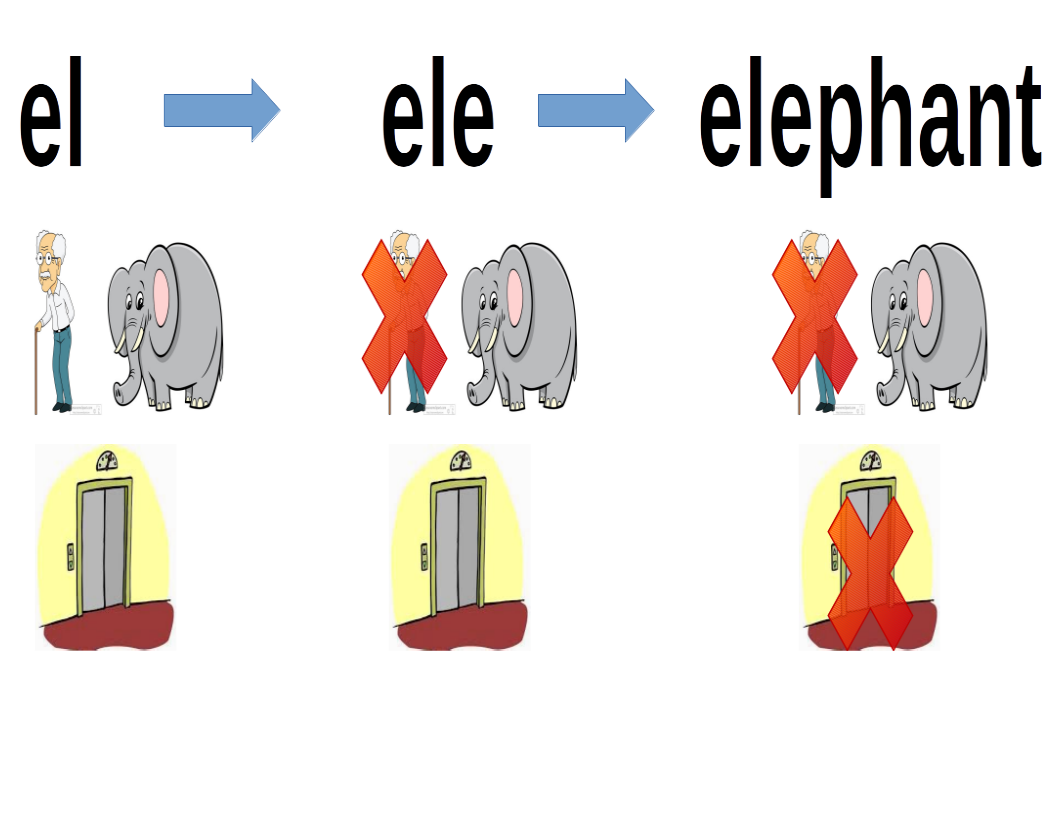
\includegraphics[scale=0.3]{img/ele_3.png}
\end{center}
\end{frame}



\begin{frame}{How does this evolve in time?} \large
Continuous mapping models of word recognition account for variety of observed phenomenon  \vp

\cn{things like immediacy (hypothesis formed from earliest input), parallelism (multiple items activated, i.e., priming), graded activation (not all-or-nothing)} \vp

In particular, connectionist models of lexical access (such as TRACE):
\begin{itemize}
\item Network structure \cn{relies on information between levels, i.e., phonemes, words, etc.)}
\item Processes in real time \cn{along with network structure, accommodates competition}
\item Nodes, activation, and signal \cn{metaphors that motivate language used to describe it}
\end{itemize}
\end{frame}



% what does trace look like
\begin{frame}
\begin{center}
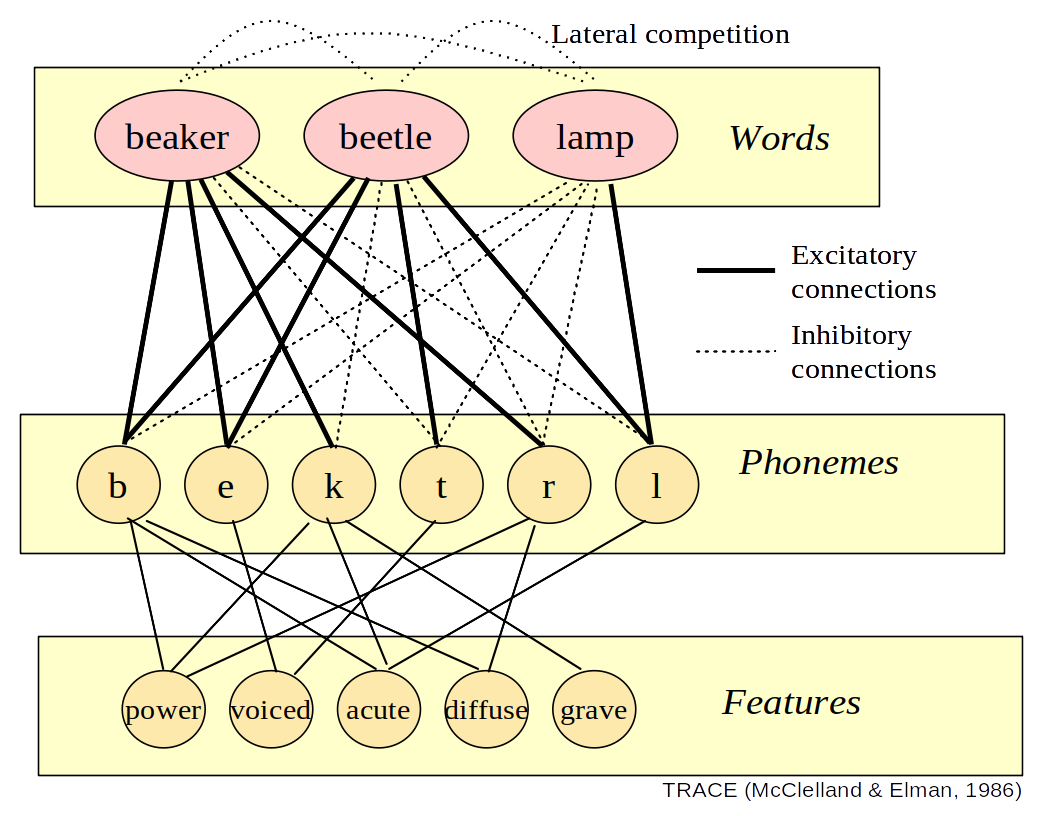
\includegraphics[scale=0.4]{img/trace_competition.png}
\end{center}
\end{frame}

\begin{frame}
\begin{figure}
\centering
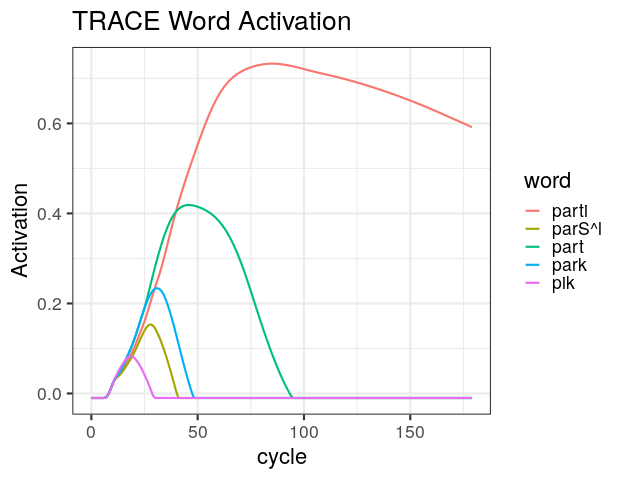
\includegraphics[scale=0.5]{img/trace_plot.png}
\caption{gave up on reordering the legend}
\end{figure}
\end{frame}

\begin{frame}
\begin{figure}
\centering
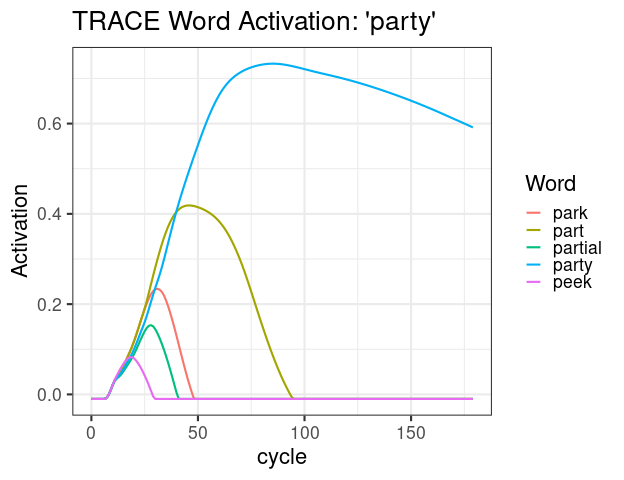
\includegraphics[scale=0.5]{img/trace_plot_reg.png}
\caption{gave up on reordering the legend}
\end{figure}
\end{frame}


% why is this important?
\begin{frame}{Why do we care?}

Typically interested in comparing activation between groups or conditions \vspace{2mm}

\begin{itemize}
\item Normal Hearing (NH) vs Cochlear Implants (CI) \vspace{2mm}
\item Differentiating cognitive, specific, and non-specific impairments \vspace{2mm}
\item Phonological perceptions \vspace{2mm}
\end{itemize}

Fortunately there is expertly written software to help accomplish this

\cn{comment that we will discuss bdots in  more detail at end}

\end{frame}

\begin{frame}{What's in a look?}

\begin{columns}
\begin{column}{0.45\textwidth}

\cn{maybe make picture larger and remove all words?}

Cognitive activation is not something that can be measured directly \vspace{4mm}

Our eyes reveal a terrifying amount of information about what we are considering \vspace{4mm}

This has been empirically tested and confirmed in countless experiments
\end{column}
\begin{column}{0.5\textwidth}
\begin{center}
%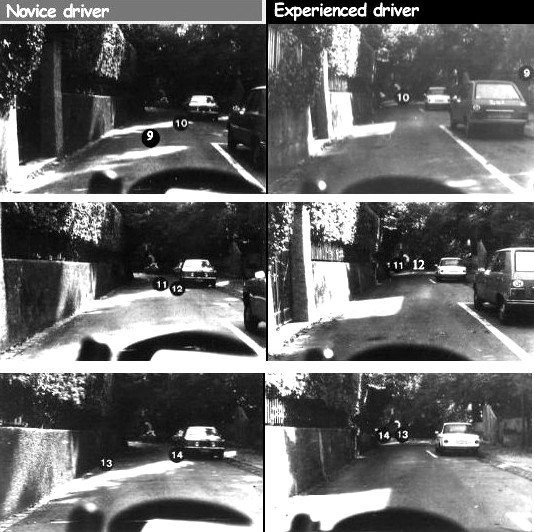
\includegraphics[scale=0.45]{img/car_eye.jpg}
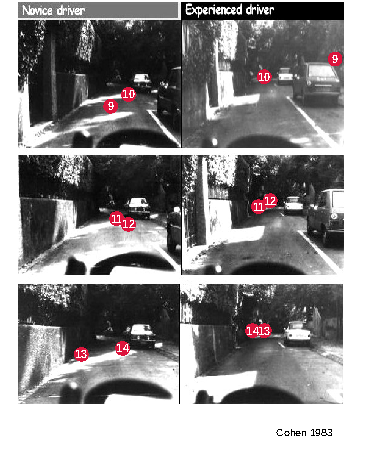
\includegraphics[scale=0.95]{img/edit_car_eye.pdf}
{\tiny Cohen 1983}
\end{center}
\end{column}
\end{columns}

\end{frame}

\begin{frame}{What's in a look?}
\vspace{-1mm}
\begin{figure}
\centering
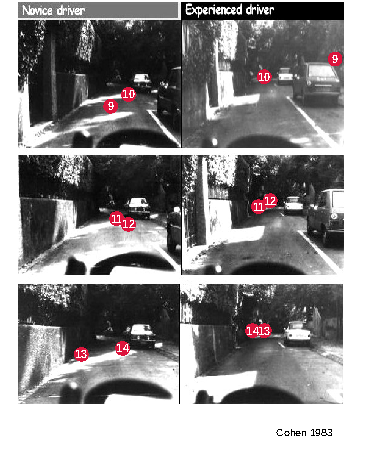
\includegraphics[scale=0.95]{img/edit_car_eye.pdf}
\caption{ what it would look like without words}
\end{figure}
\end{frame}



\begin{frame}{Visualizing Eye Mechanics}
\vspace{-1mm}
\begin{figure}
\centering
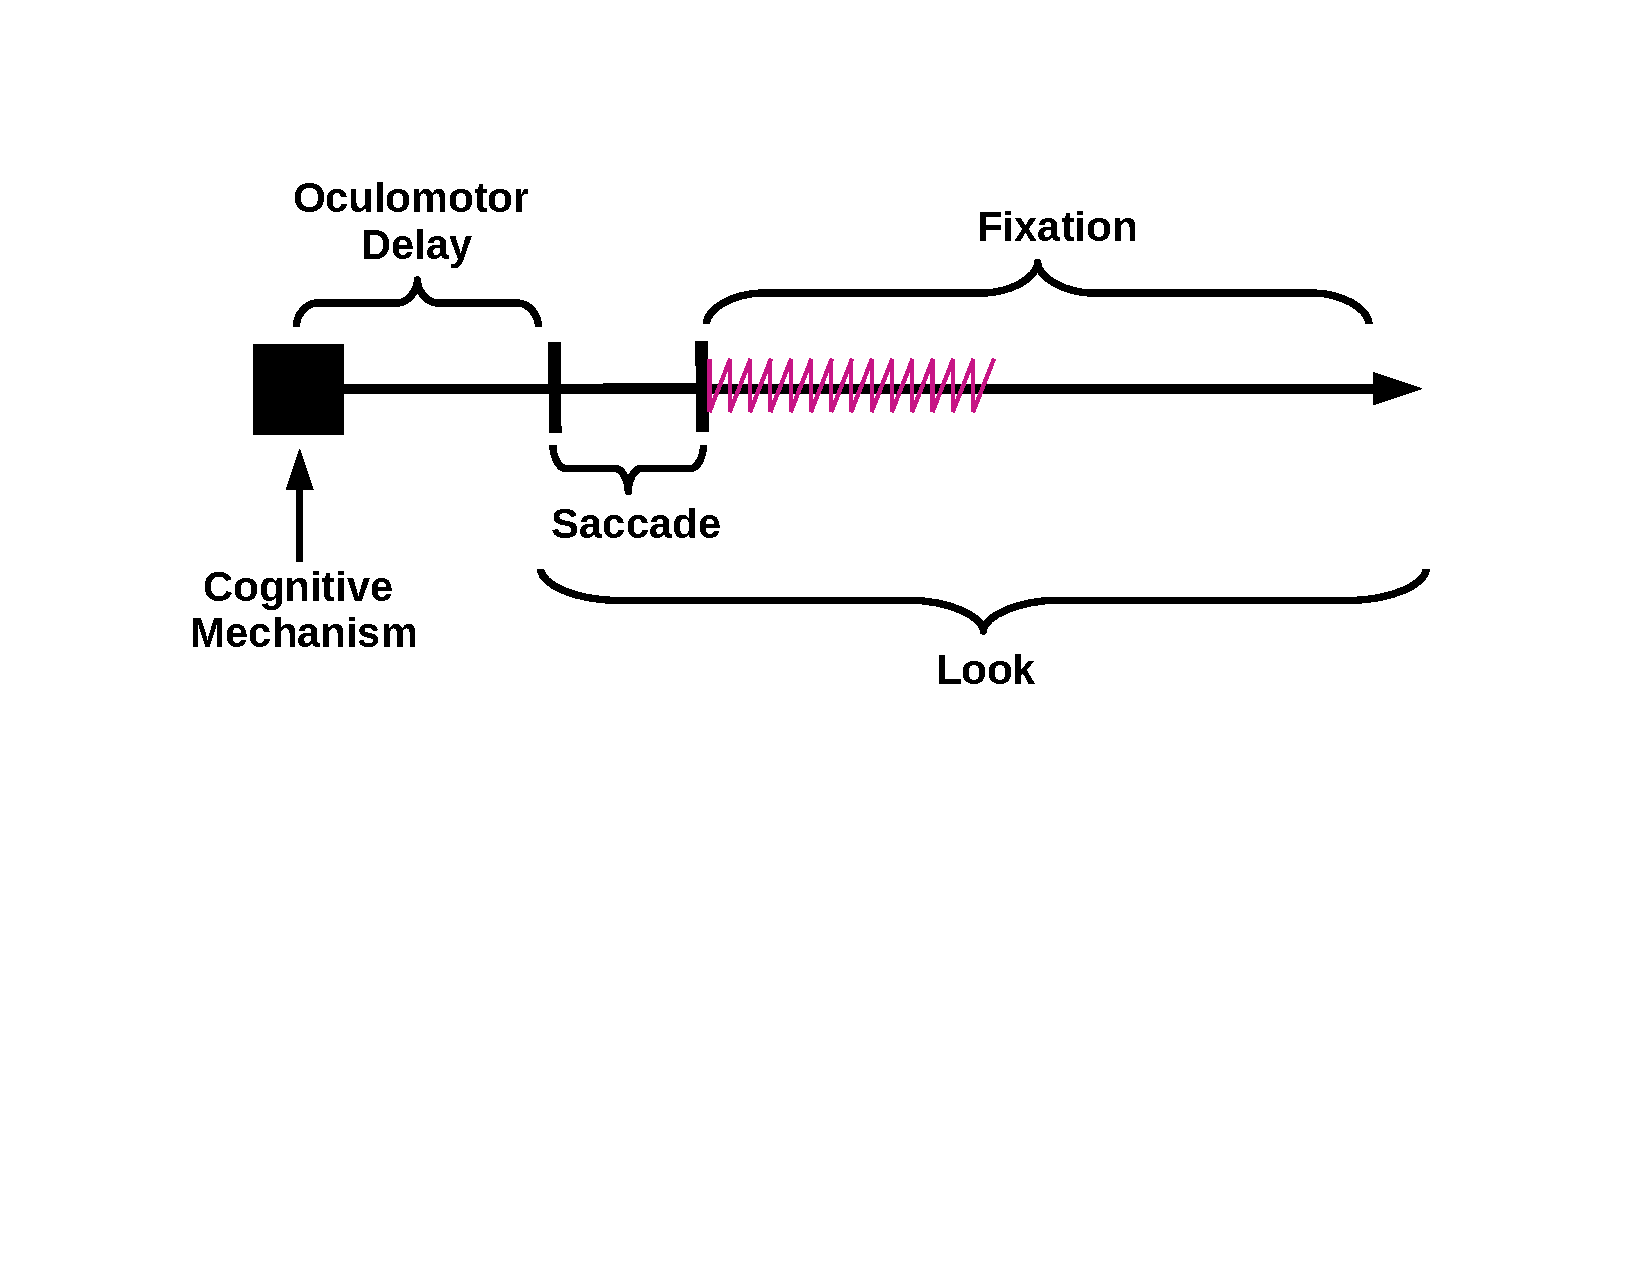
\includegraphics[scale=0.45]{img/what_is_a_look.pdf}
\caption{just describe this with words, mention 200ms delay, etc)}
\end{figure}
\end{frame}




% Enter vwp
\begin{frame}{Visual World Paradigm}
\begin{columns}
\begin{column}{0.45\textwidth}

Visual World Paradigm introduced in 1995 \vp

Eye-tracking in conjunction with spoken sentence \vp

``The boy will move the cake" \vp

How do we go from this to word recognition? \vp

\cn{talk about differential eye tracking with ambiguity, etc (maybe use that image instead)}
%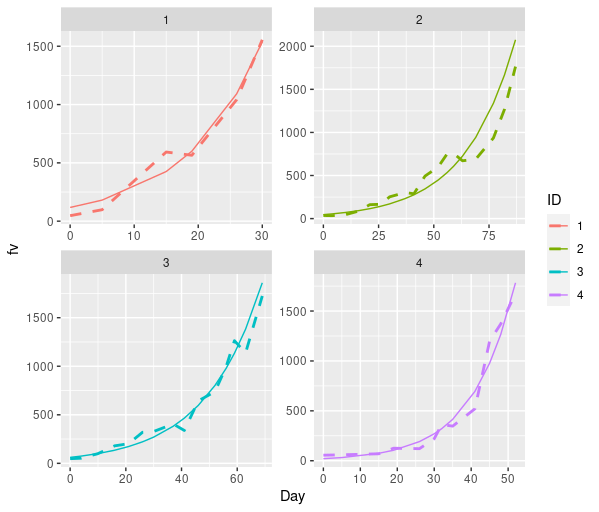
\includegraphics[scale=0.45]{img/tumr_fit.png}

\end{column}
\begin{column}{0.5\textwidth}  %%<--- here
\begin{center}
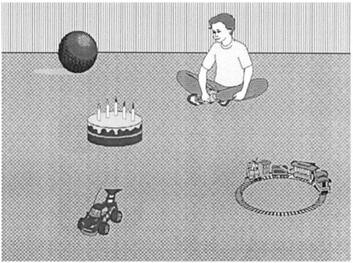
\includegraphics[scale=.9]{img/vwp_classic.png}
\end{center}
\end{column}
\end{columns}
\end{frame}

\begin{frame}{alt image for vwp}
\begin{figure}
\centering
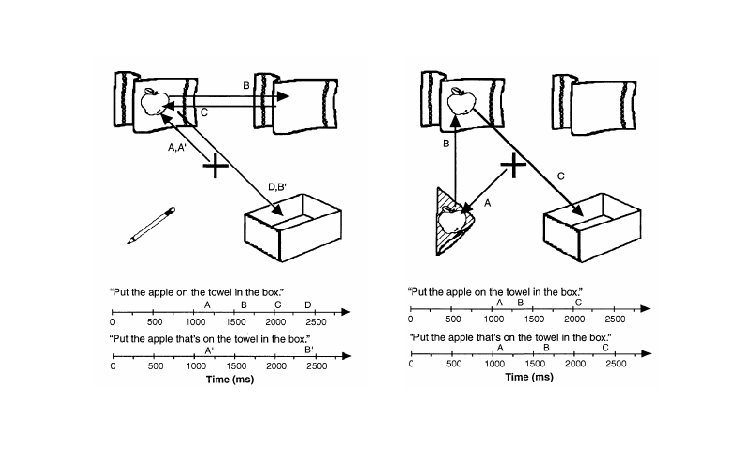
\includegraphics[width=\textwidth]{apple_combine.pdf}
%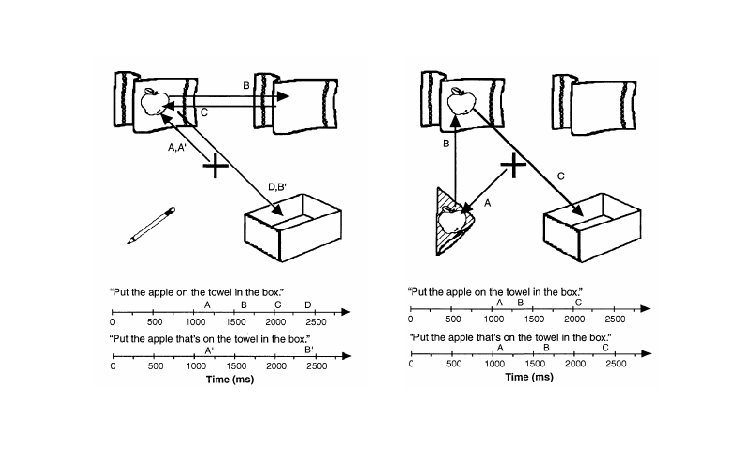
\includegraphics[scale = 1.1]{apple_combine.pdf}
\caption{Differential eye response based on context and ambiguity}
\end{figure}
\end{frame}



\begin{frame}{VWP Trials}
\begin{center}
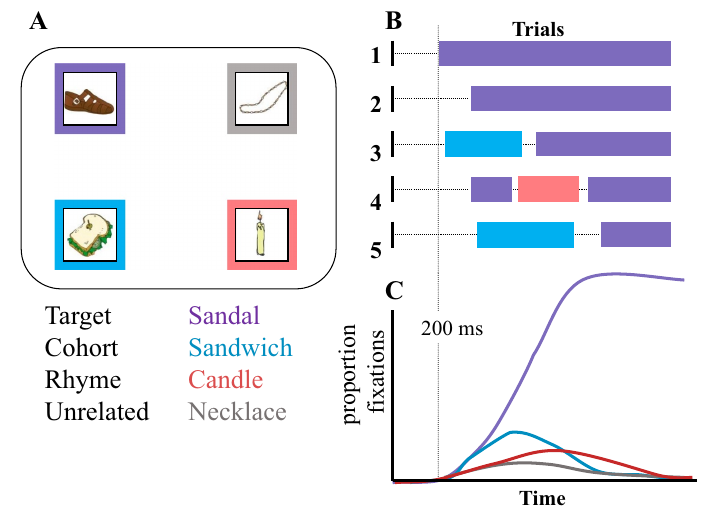
\includegraphics[scale=0.4]{img/bob_vwp_full.png}
\end{center}
\end{frame}

% just image from allopenna, magnuson and tanenhaus 
\begin{frame}{Original study}
\begin{center}
% screenshot from paper
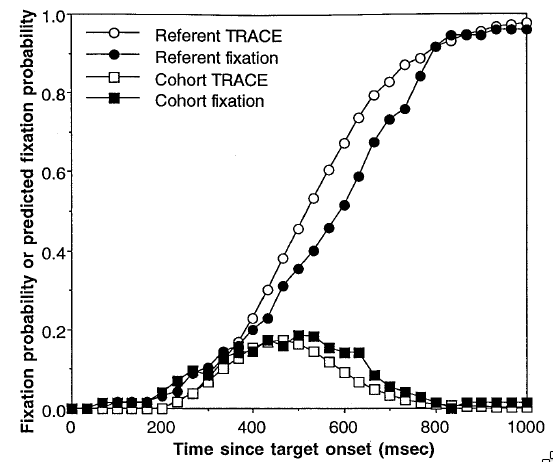
\includegraphics[scale=0.45]{img/allopenna_trace_compare.png}
\end{center}
\end{frame}


% how related to vwp
\begin{frame}{So how does this relate to VWP}

\begin{columns}
\begin{column}{0.45\textwidth}
To make the problem more tractable, curves given a (usually) parametric form, $f_{\theta}(t)$ or $f(t| \theta)$ \\ \vspace{2mm}

Letting $z_{ijt}$ represent fixation at time $t$ for trial $j$, we have empirical curve
\begin{align*}
y_{it} = \sum_j z_{ijt}
\end{align*}
and find
\begin{align*}
\hat{\theta} = \argmin_{\theta} \mathcal{L}(f_{\theta}, y)
\end{align*}

\end{column}
\begin{column}{0.5\textwidth}  %%<--- here
\begin{center}
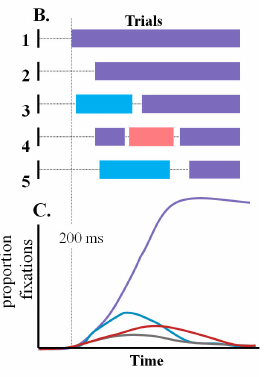
\includegraphics[scale=0.5]{img/bob_aggregate.png}
\end{center}
\end{column}
\end{columns}
\end{frame}


\begin{frame}{Parametric Function}

\vspace{-5mm}

\begin{columns}
\begin{column}{0.45\textwidth}
Here, for example, is a four-parameter logistic function, typically used for the referent: \vspace{5mm}
\begin{align*}
f_{\theta}(t) = b + \frac{p-b}{1 + \exp \left( \frac{4s}{p-b} (c - t) \right)}
\end{align*}
%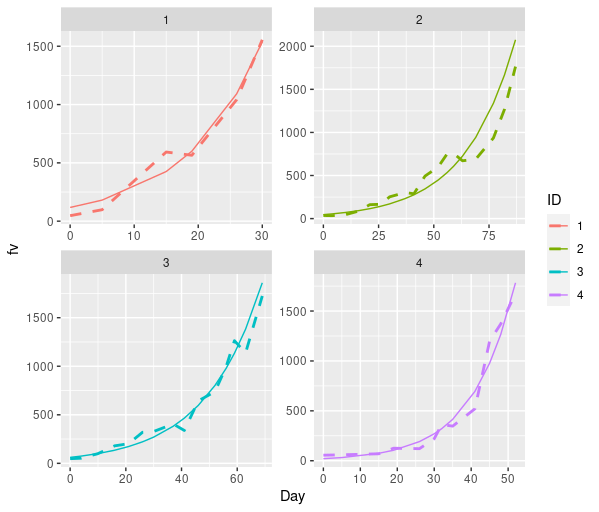
\includegraphics[scale=0.45]{img/tumr_fit.png}
\end{column}
\begin{column}{0.5\textwidth}  %%<--- here
\begin{center}
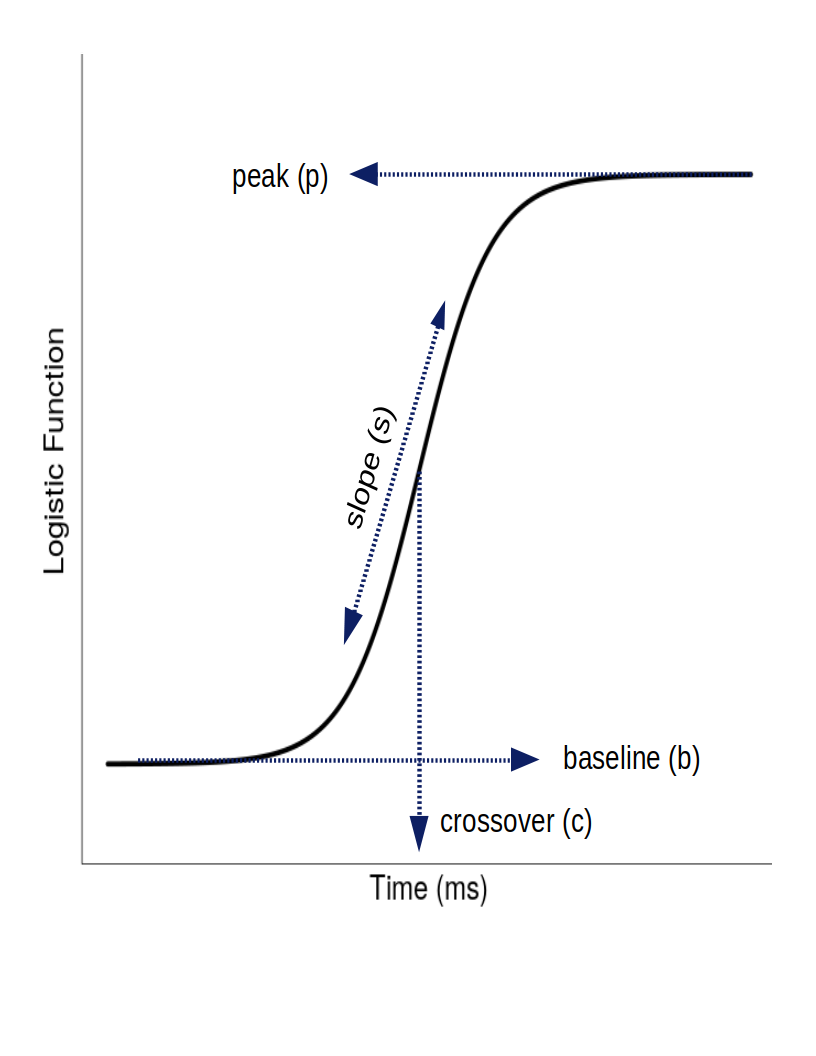
\includegraphics[scale=0.3]{img/logistic_label.png}
\end{center}
\end{column}
\end{columns}
\end{frame}

\begin{frame}{Linking hypothesis}\Large

Have used $f(t|\theta)$ as functional form for proportion of fixations, but relation to activation still implicit/undefined \vp

\cn{``The default interpretation is greater fixation proportions indicate greater activation in the underlying processing system" (Magnuson 2019)} \vp


Our primary proposal is that it is the underlying activation, rather than observed data, that should be modeled explicitly as $f(t|\theta)$ \vp

%Under this proposal, there are major issues with proportion of fixation method

\end{frame}

\begin{frame}{Issues}

\cn{Actually, let's move delay observation bias until \textit{after} look onset introduced since its unrelated, but relevant for sim}

\cn{maybe move illustration of saccade/OM/fixation to immediately after this slide?}

\cn{in light of this...} Despite visual similarities between the proportion of fixations and activation, there is an issue with the equivalence

\begin{align*}
y_{it} \equiv f(t | \theta_i)
\end{align*}

Eye mechanics made up of distinct mechanisms that are differentially related to activation \vp

\cn{maybe don't specifically say anything here, save discussion for next slide then move on to added observation bias}

\end{frame}

\begin{frame}{Visualizing Eye Mechanics}
\vspace{-1mm}
\begin{figure}
\centering
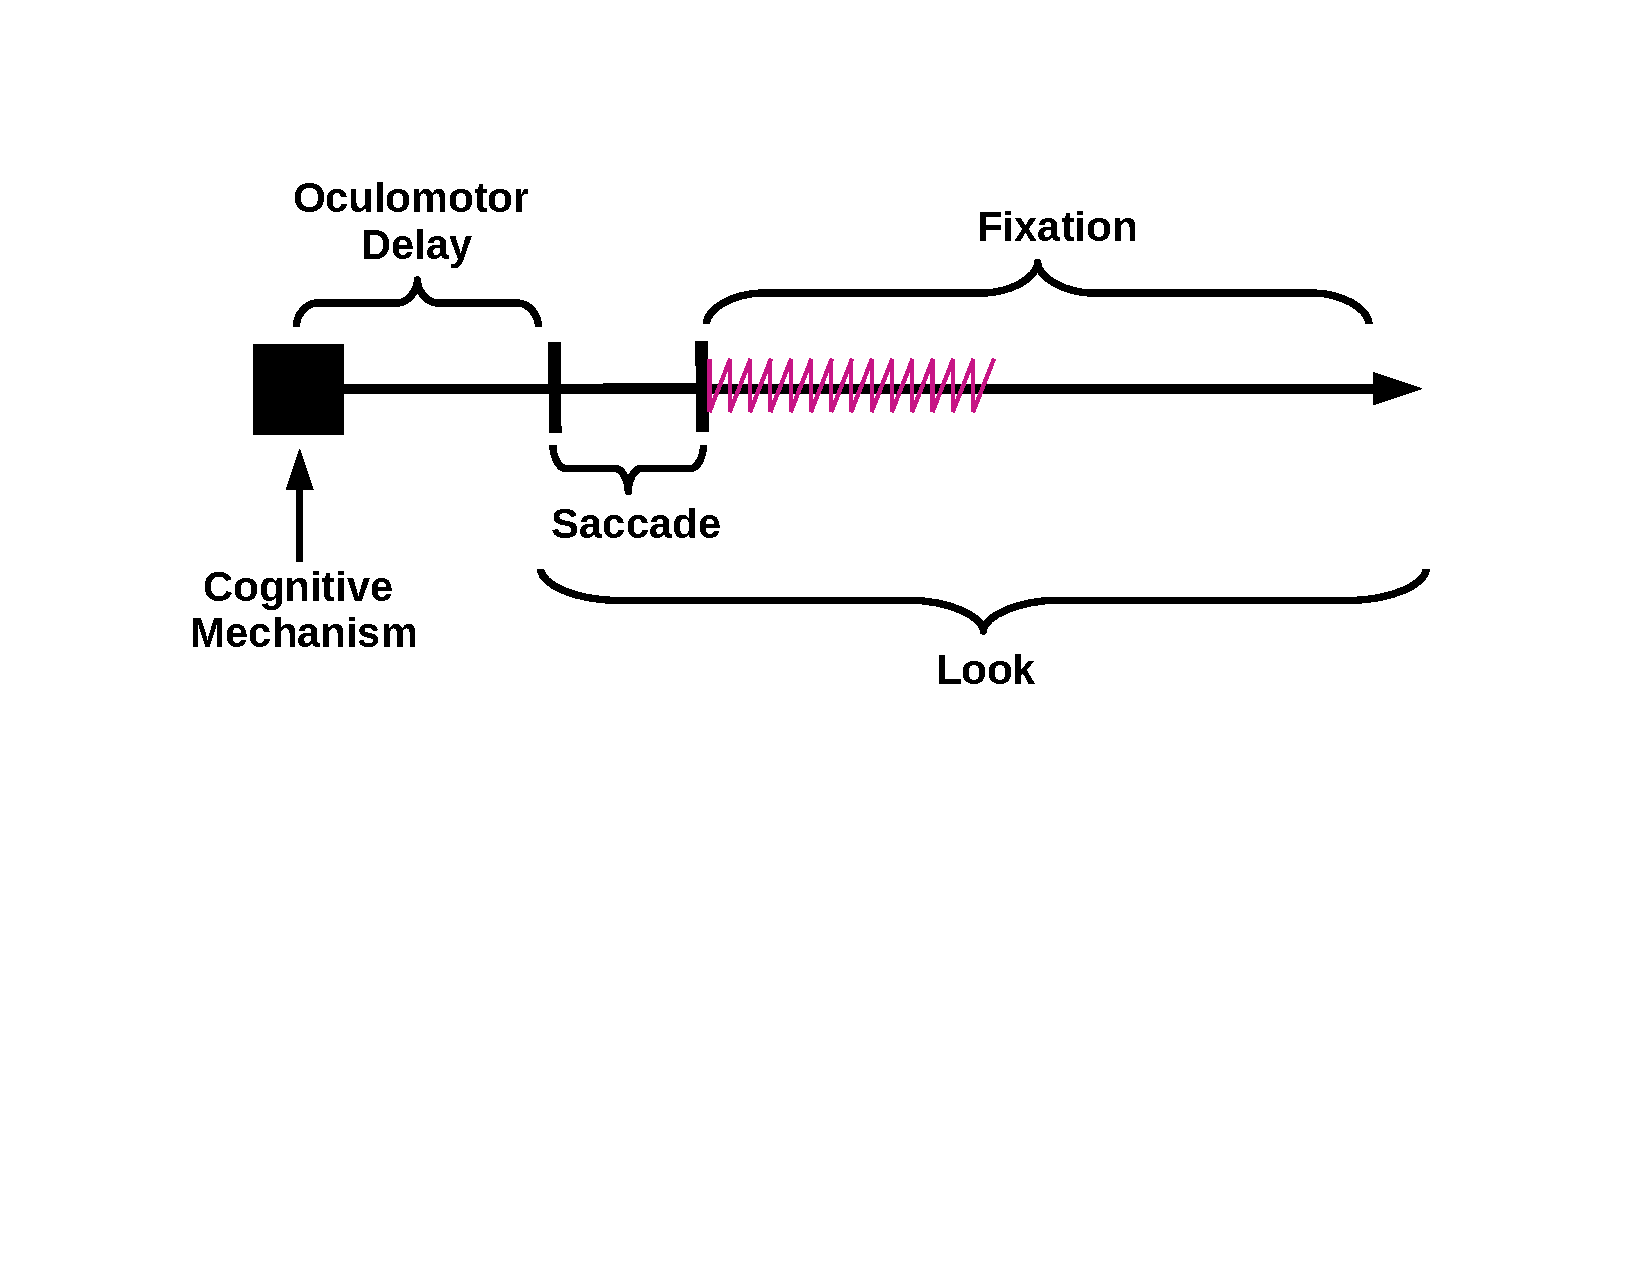
\includegraphics[scale=0.45]{img/what_is_a_look.pdf}
\caption{just describe this with words, mention 200ms delay, etc)}
\end{figure}
\end{frame}


%
%\begin{frame}{Issues (another attempt)}
%We are predominately interested in the recovery of a lexical activation function, though given visual similarities between the proportion of fixations and activation, we have the ostensible equivalence, 
%
%\begin{equation}
%y_{it} \equiv f(t | \theta_i)
%\end{equation}
%
%There are primarily two sources of biases inherent in this method which hitherto have been left unexamined:
%
%\begin{itemize}
%\item[1.] Delayed observation bias/error
%\item[2.] Added observation bias
%\end{itemize}
%
%\cn{(in reverse order because easier to explain plus its mostly an aside)}
%\end{frame}


\begin{frame}{Added Observation Bias}

\cn{too many words} \vp

Added observation bias arises from the conflation of two distinct (though likely correlated) processes: the decision to initiate an eye movement to a particular place and the duration of a fixation\vp

\cn{We are interested in the process that probabilistically determines the \textit{location} of a fixation} \vp

\cn{At some time $t$, a saccade is launched, and we know from length of saccade until \textit{at least} refractory period for fixation, it is impossible for our eyes to go anywhere else} \vp

By including the entire length of the fixation as ``observed" data relating to this process, we are both inflating the amount of data we have with data that is necessarily biased
\end{frame}


\begin{frame}{Activation curve}
\vspace{-5mm}
\begin{center}
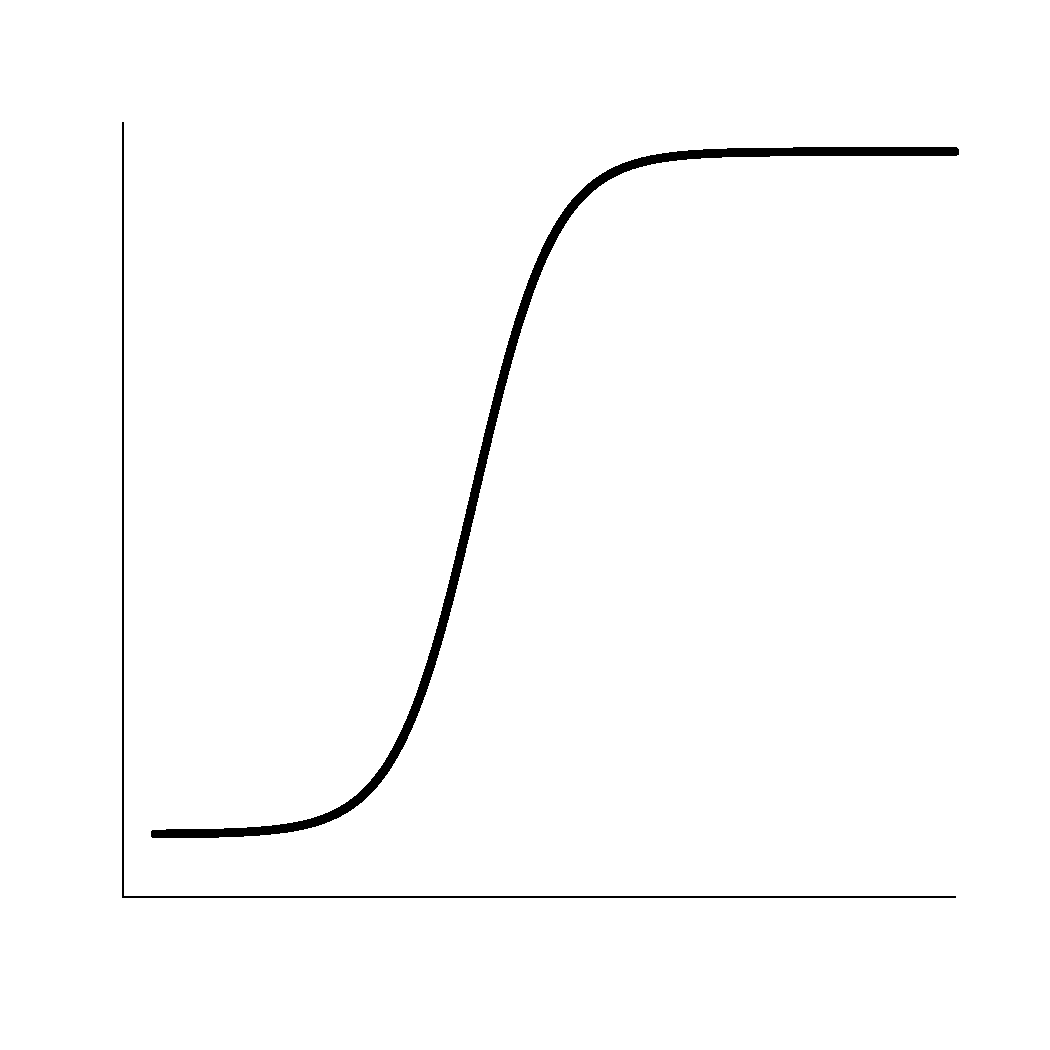
\includegraphics[scale=0.4]{img/logistic_a.pdf}
\end{center}


\end{frame}

\begin{frame}{Onset of look}
\vspace{-5mm}
\begin{center}
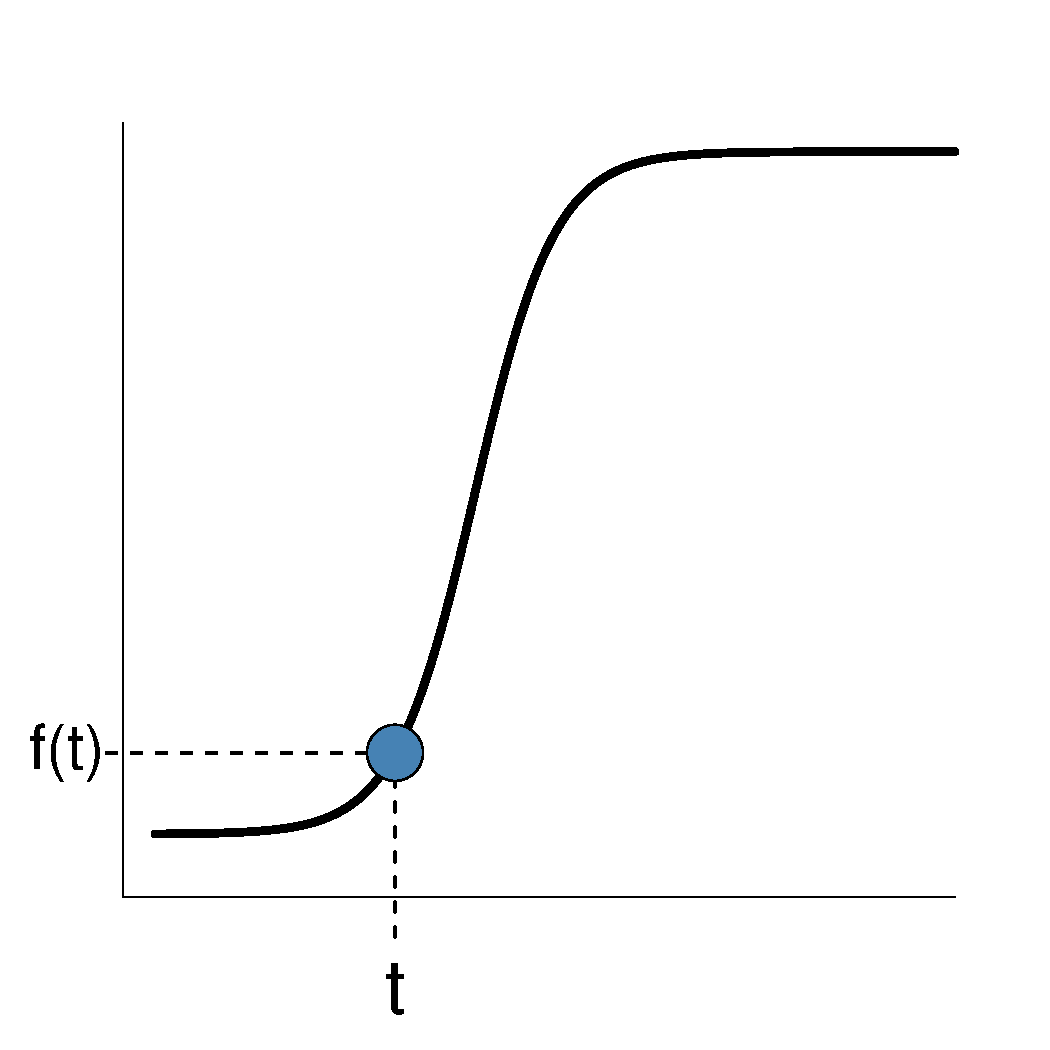
\includegraphics[scale=0.4]{img/logistic_b.pdf}
\end{center}

\end{frame}

\begin{frame}{...followed by fixation}
\vspace{-5mm}
\begin{center}
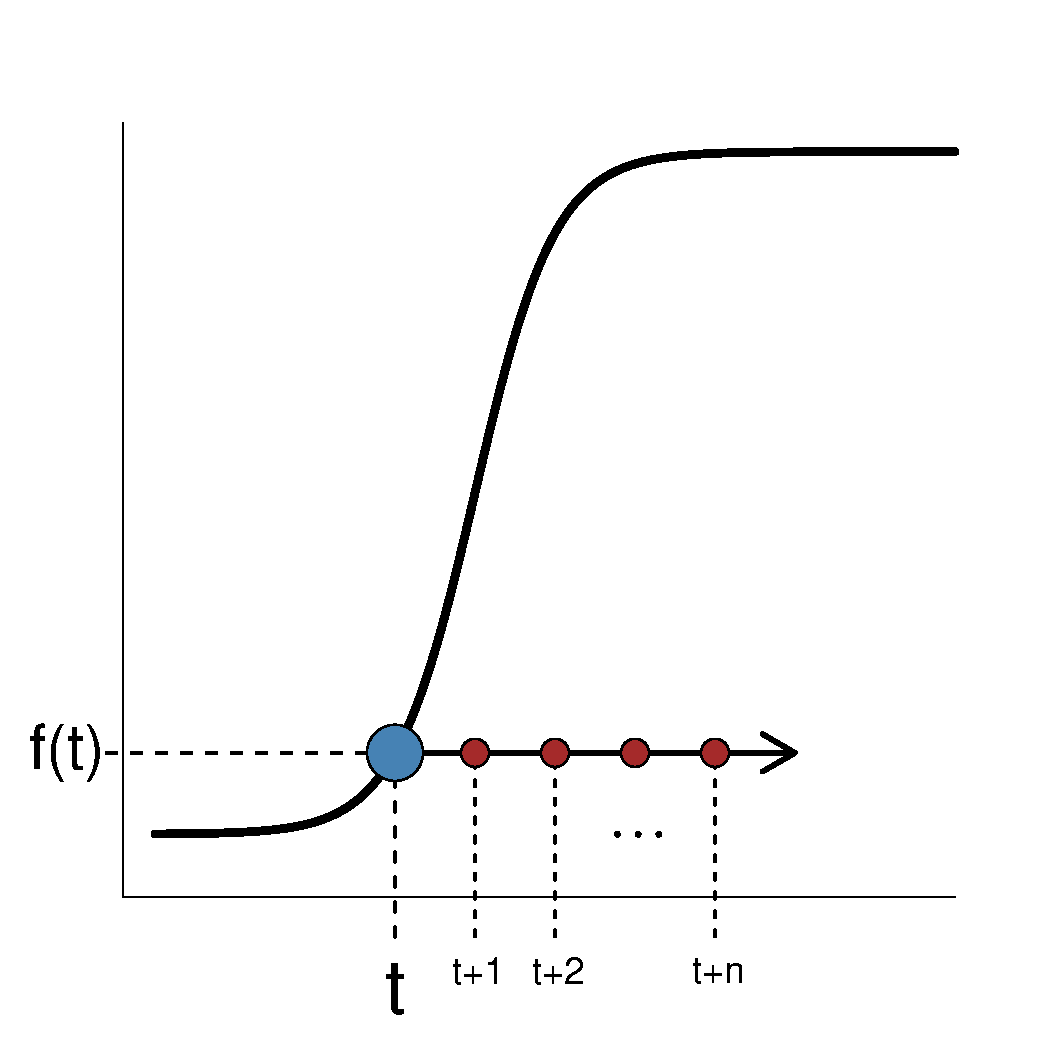
\includegraphics[scale=0.4]{img/logistic_c.pdf}
\end{center}
\end{frame}

\begin{frame}{Look Onset Method}
\cn{As the cognitive mechanism responsible for initiating an eye movement is probabilistically (allopenna) related to activation, we argue that the instance of a look onset is a more theoretically consistent and physiologically defensible observation to treat as relevant data} \vp

\cn{We propose look onset method}

Only the initial moment of look onset, $s_j$, is considered relevant in the recovery of latent activation, where a look initiated at time $t_j$ follows
\vspace{-2mm}
%\begin{equation}
%s_j \sim Bern \left[f(t_j | \theta)\right]
%\end{equation}

\begin{align*}
s_j \sim Bern \left[f(t_j | \theta)\right]
\end{align*}

This gives us instead a set of ordered pairs, $\mathcal{S} = \{(s_j, t_j)\}$ rather than a time ordered vector of proportions \\ \vp

Fortunately, we are able to use nearly an identical procedure as before, 
\begin{align*}
\hat{\theta} = \argmin_{\theta} \mathcal{L}(f_{\theta}, \mathcal{S})
\end{align*}

\end{frame}

%\begin{frame}{Look Onset Method}
%\cn{As the cognitive mechanism responsible for initiating an eye movement is probabilistically (allopenna) related to activation, we argue that the instance of a look onset is a more theoretically consistent and physiologically defensible observation to treat as relevant data} \vp
%
%Under the look onset method, only the initial moment of look onset, $s_j$, is considered relevant in the recovery of latent activation, where a look initiated at time $t_j$ follows
%
%\begin{align*}
%s_j \sim Bern(f_{\theta}(t_j))
%\end{align*}
%
%This gives us instead a set of ordered pairs, $\mathcal{S} = \{(s_j, t_j)\}$ rather than a time ordered vector of proportions \\ \vp
%
%Fortunately, we are able to use nearly an identical procedure as before, 
%\begin{align*}
%\hat{\theta} = \argmin_{\theta} \mathcal{L}(f_{\theta}, \mathcal{S})
%\end{align*}
%\end{frame}


\begin{frame}{Delayed Observation}\large

Between the cognitive mechanism \cn{probabilistically related to activation} and the initiation of look onset is a period of oculomotor delay, $\rho$ \vp

This gives distribution of look onset,
\vspace{-1mm}
\begin{align*}
s_j \sim Bern \left[f(t_j - \rho) | \theta)\right]
\end{align*}

It is ``roughly" estimated to be around 200ms, and this is typically accounted for by subtracting 200ms from observations \vp

\cn{Of course any actual bias would be the difference between the true value and the 200ms subtracted, but also has been no treatment as to the effect of randomness} \vp

We show that varying degrees of randomness in this process and drastically impact error in recovery

\end{frame}
%
%\begin{frame}{Delayed Observation}\large
%
%\cn{too many words} \vp
%
%Delayed observation bias arises from the oculomotor delay between the cognitive process (of interest) and the first physiological response, denote $\rho$ \vp
%
%It is ``roughly" estimated to be around 200ms, and this is typically accounted for by subtracting 200ms from observations \vp
%
%\cn{Of course any actual bias would be the difference between the true value and the 200ms subtracted, but also has been no treatment as to the effect of randomness} \vp
%
%We show that varying degrees of randomness in this process and drastically impact error in recovery
%\end{frame}

\begin{frame}{Simulation}\Large

Create simulated VWP trials with eye mechanics with goal of recovering activation curve, $f(t|\theta)$ \vp \vp

Each subject draws individual $\theta_i$ \cn{from empirically determined distribution} and will perform 300 trials. 1,000 total subjects \vp \vp

Metric for efficacy is MISE between generating function and recovered curve using \xt{bdots}
\end{frame}


\begin{frame}{Simulation -- Single Trial}\large
\cn{Will need to fill in with exposition, don't want dense text on slide}

\cn{Alternatively, I could just skip a slide like this all together and just explain in picture}

\begin{enumerate}
\item[1.] Look initiated at $t_0$, persisting for at least duration $\gamma$
\item[2.] At $t_0 + \gamma$, look towards target with probability $f(t_0 + \gamma|\theta)$
\item[3.] This is followed by oculomotor delay, $\rho$
\item[4.] At $t_0 + \gamma + \rho$, current look ends and next is immediately initiated
\end{enumerate}

\vspace{5mm}

A trial begins at $t = 0$ and continues until the cumulative duration of looks within trial exceeds 2000ms

\cn{would also say here or next slide we run three types with various distributions of $\rho$}

\end{frame}

\begin{frame}{Simulation (explain in words, could have less detail here)}

\vspace{-2.5mm}
\begin{figure}
\centering
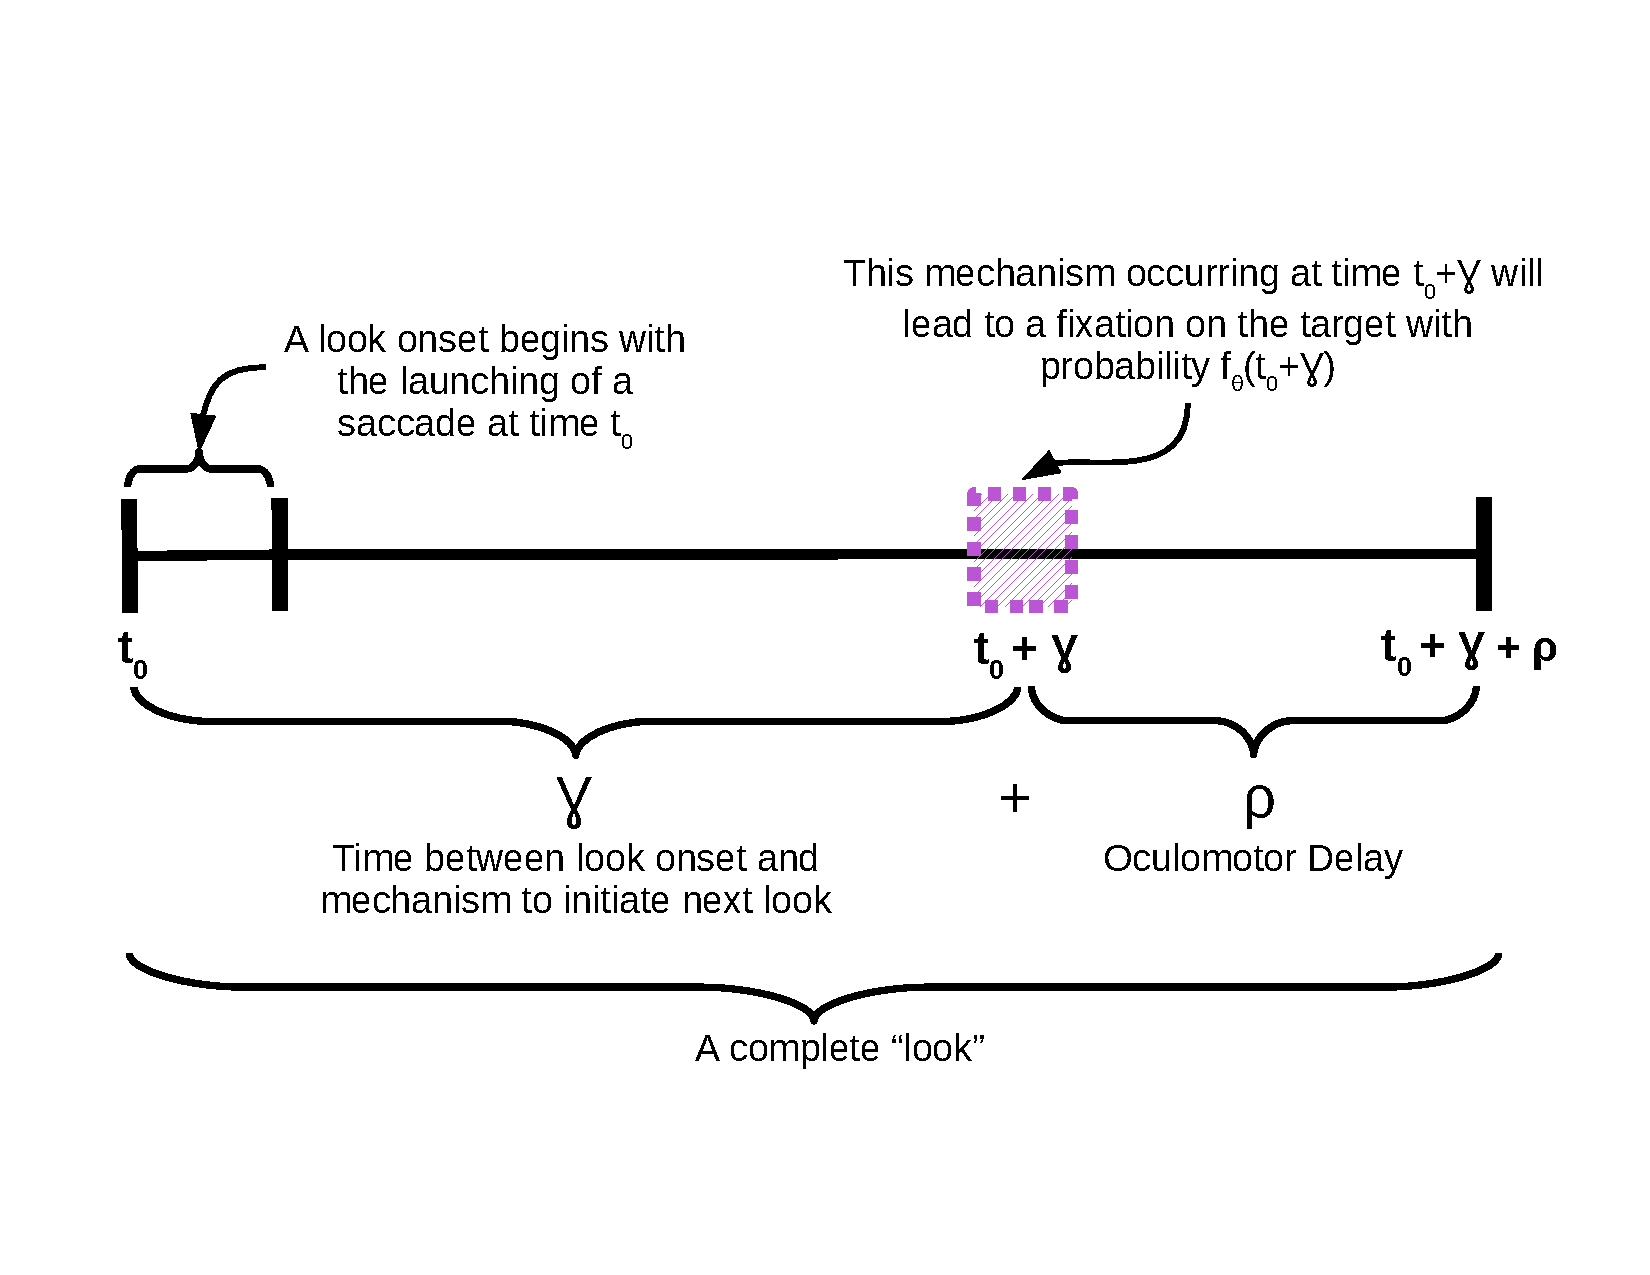
\includegraphics[scale=0.4]{look_comp.pdf}
\end{figure}
\end{frame}

\begin{frame}{notes on results section}
[all meta commentary here, will delete slide] \vp

Probably not necessary to include all simulations, I'll just choose two \vp

I can make the proportion curves look as good or bad as I want by modifying  the $\gamma$ parameter. I don't think that's necessary here as I can comment as to why small changes make a large difference in subsequent analysis \vp

For weibull delay, im only going to compare par bias for onset method against no delay since after the first sim there is really no reason to look at proportion method again
\end{frame}


\begin{frame}
\begin{figure}[H]
\centering
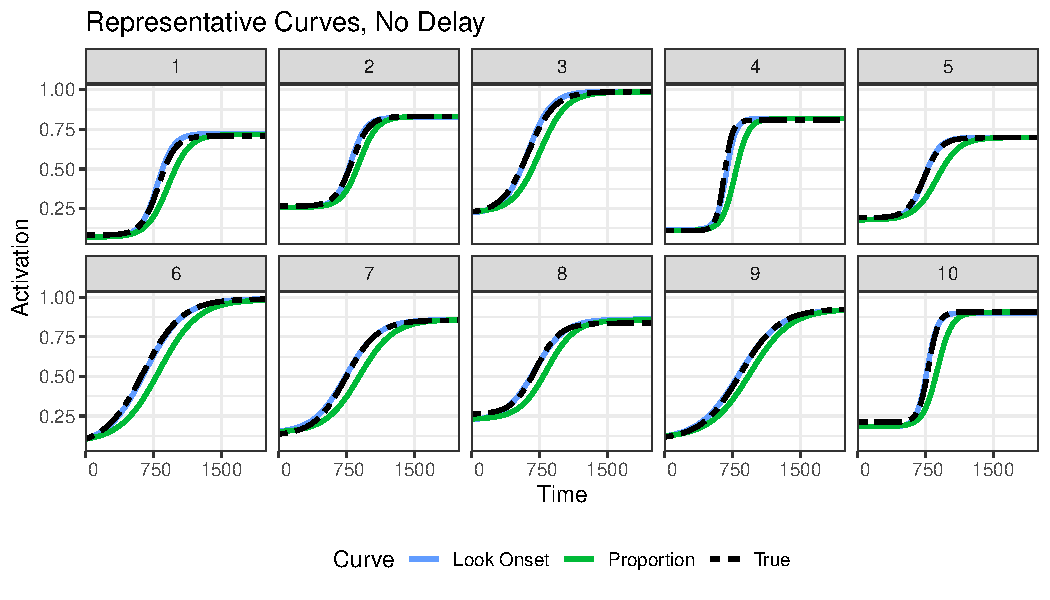
\includegraphics[width=0.9\textwidth]{rep_curves_no_delay.pdf}
\caption{Representative curves with no oculomotor delay}
\label{fig:rep_curves_no_delay}
\end{figure}
\end{frame}


\begin{frame}
\begin{figure}[H]
\centering
    \subfigure{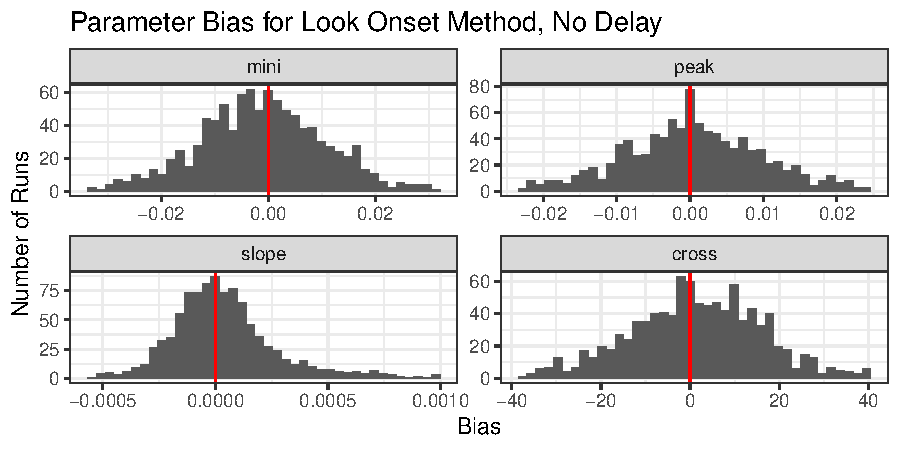
\includegraphics[width=0.6\textwidth]{no_delay_par_bias_onset.pdf}} 
    \subfigure{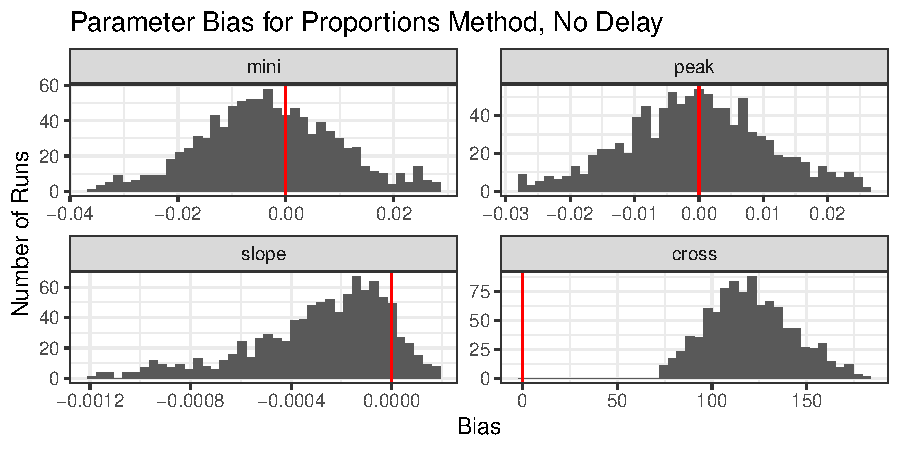
\includegraphics[width=0.6\textwidth]{no_delay_par_bias_proportion.pdf}} 
\caption{Parameter bias with no oculomotor delay}
\label{fig:par_bias_no_delay}
\end{figure}
\end{frame}



\begin{frame}
\begin{figure}[H]
\centering
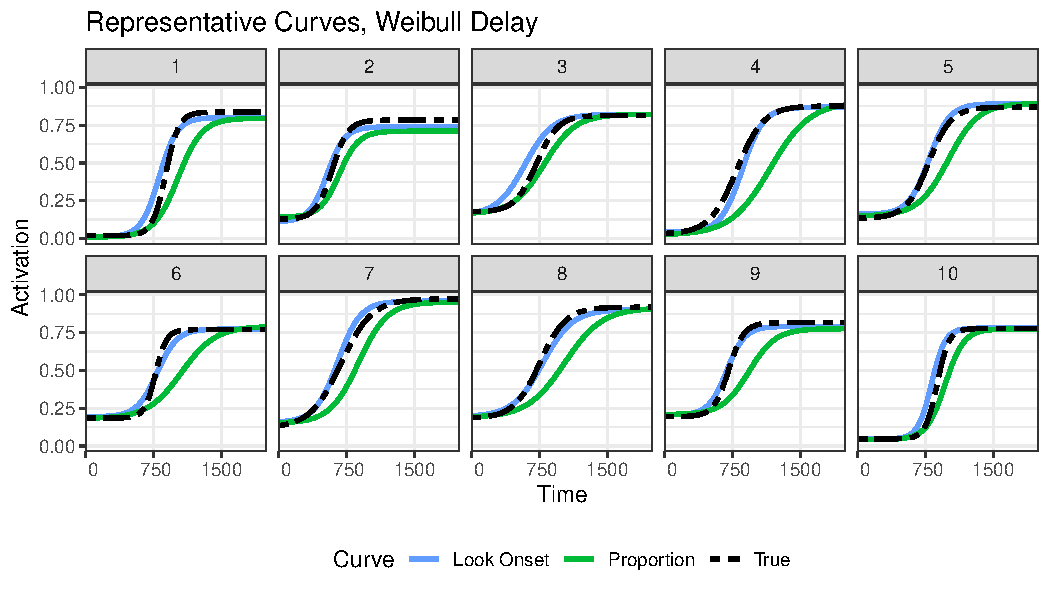
\includegraphics[width=0.9\textwidth]{rep_curves_weibull_delay.pdf}
\caption{Representative curves with no Weibull delay}
\label{fig:rep_curves_no_delay}
\end{figure}
\end{frame}


\begin{frame}
\begin{figure}[H]
\centering
    \subfigure{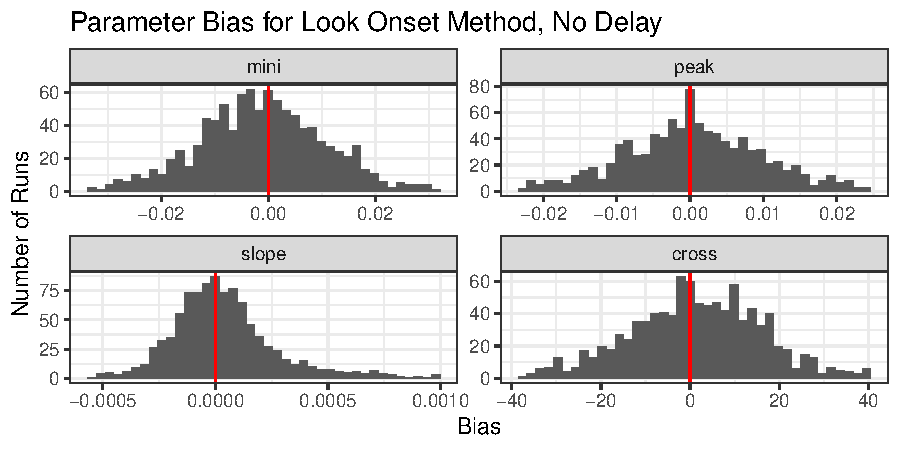
\includegraphics[width=0.6\textwidth]{no_delay_par_bias_onset.pdf}} 
    \subfigure{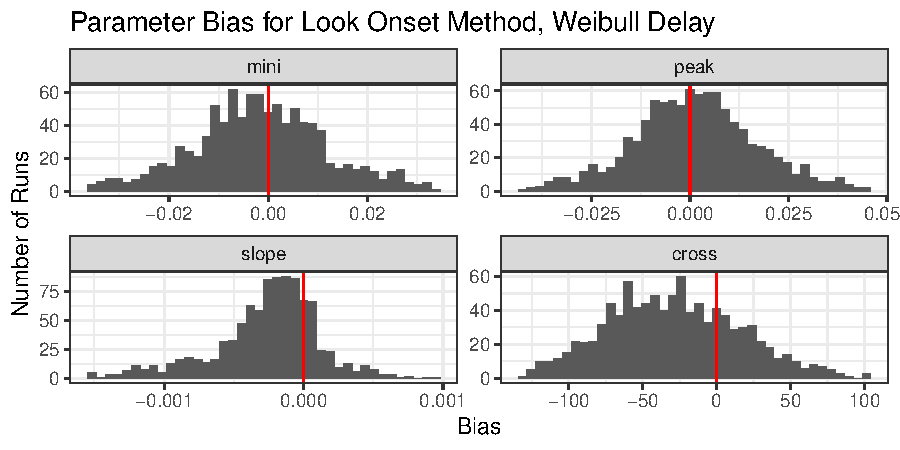
\includegraphics[width=0.6\textwidth]{weibull_delay_par_bias_onset.pdf}} 
\caption{Parameter bias for look onset method}
\label{fig:par_bias_no_delay}
\end{figure}
\end{frame}

\begin{frame}{MISE}

\begin{table}[H]
\centering
\begin{tabular}{llrrr}
  \hline
Method & Delay & 1st Qu. & Median & 3rd Qu. \\ 
  \hline
Look Onset & No Delay & 0.17 & 0.32 & 0.56 \\ 
  Look Onset & Weibull Delay & 1.05 & 2.16 & 4.23 \\ 
  Proportion & No Delay & 8.21 & 11.33 & 16.01 \\ 
  Proportion & Weibull Delay & 15.27 & 24.75 & 38.14 \\ 
   \hline
\end{tabular}
\caption{Summary of mean integrated squared error across simulations}
\label{tab:mise_sims}
\end{table}

\end{frame}

%% End with list of other things that I will be doing going forward
\begin{frame}{Where from here?}

\cn{maybe elaborate on bdots \textit{here}, what it can do, how it changed, etc.,. I also like the idea of talking a bit more about oculmotor delay (and I left that slide comparing curves after this), but its mostly theoretical time filler since I didn't actually do anything to address it}

\begin{itemize}
\item Oculomotor delay
\item \xt{bdots}
\item Simulation for eyetracking/physiology
\item Extending the model (number of saccades, search patterns, etc.,)
\end{itemize}
\end{frame}
%
%% talk about oculomotor delay
%\begin{frame}{Oculomotor delay}
%Though we talk about saccades and fixations, what we are \textit{actually} interested in is this latent cognitive mechanism
%
%It happens in our head first and then our eyes move. This delay, typically around 200ms, is random, and can bias our estimates \\
%
%We will call the length of an  oculomotor delay $\rho(t)$
%
%\begin{center}
%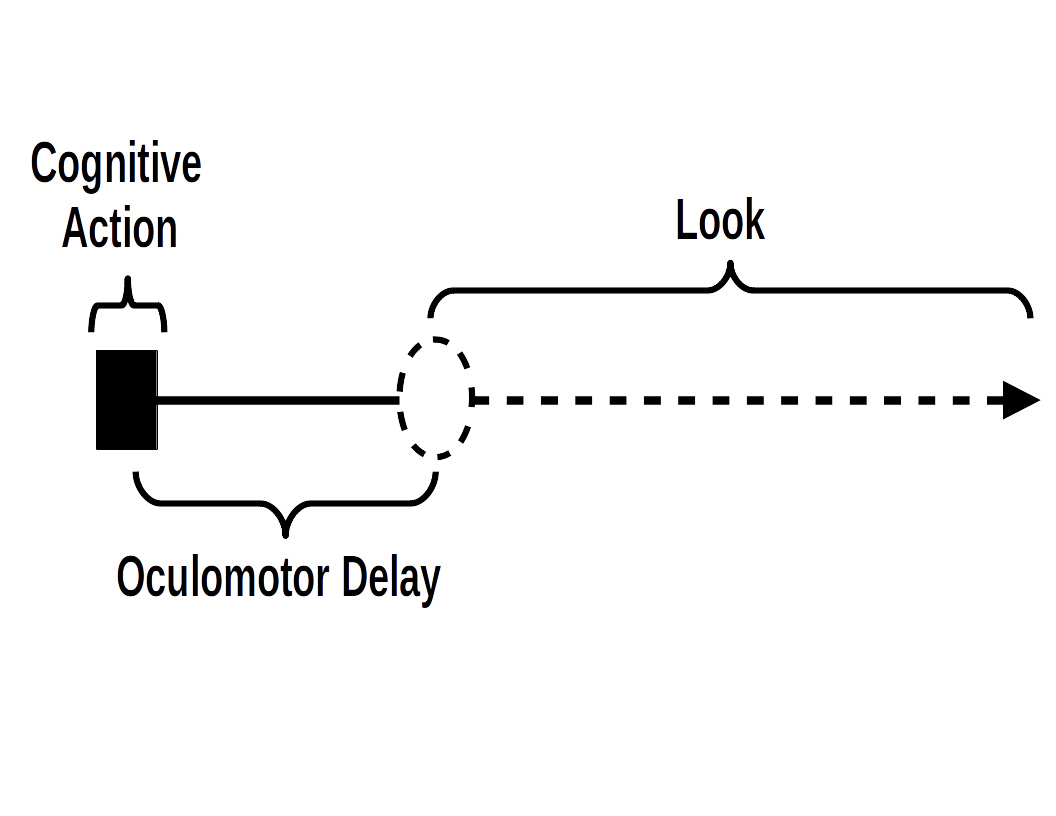
\includegraphics[scale=0.25]{img/om_delay2.png}
%\end{center}
%
%\end{frame}
%
%\begin{frame}{Oculomotor delay, cont.}
%A saccade observed at time $t_j$ is likely a sample from the activation curve $f_{\theta}$ at some point prior to $t_j$. We might then consider our saccades to be
%\begin{align*}
%s_j \sim Bern[f_{\theta}(t_j - \rho(t_j)],
%\end{align*}
%where $\rho(t)$ represents our oculomotor delay. It may be the case that:
%
%\begin{itemize}
%\item[1.] $\rho(t)$ is a constant function (including 0)
%\item[2.] $\rho(t)$ is a random variable, independent on the value of $t$
%\item[3.] $\rho(t)$ is a random variable, dependent on $t$ and possibly other aspects of the trial
%\end{itemize}
%
%For clarity, then, we might call $f_{\theta}(t)$ the (latent) activation curve, with $g_{\theta}(t) = f_{\theta}(t - \rho(t))$ our (observed) saccade curve
%
%\end{frame}
%
%
\begin{frame}{Impact of random delay}
\begin{center}
% code for doing this in dissertation folder
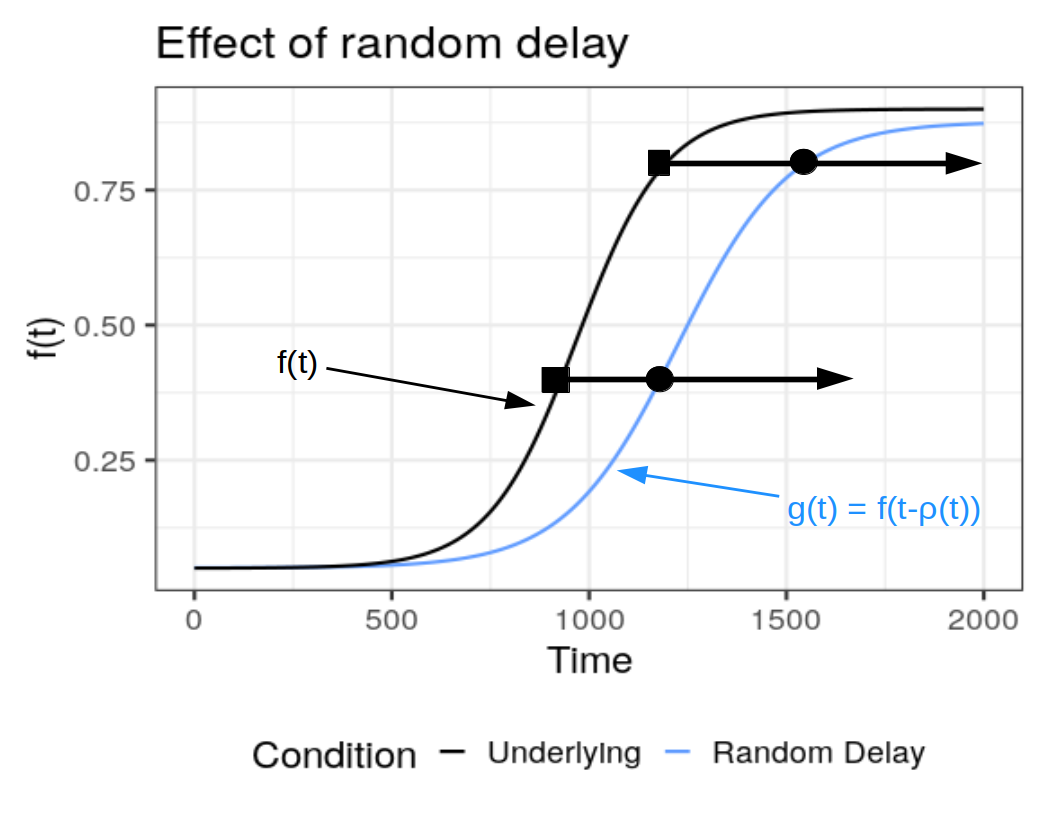
\includegraphics[scale=0.35]{img/full_delay_plot.png}
\end{center}
\end{frame}


\begin{frame}{Bootstrapped differences in time series -- \texttt{bdots}}
\vspace{-1mm}
\begin{center}
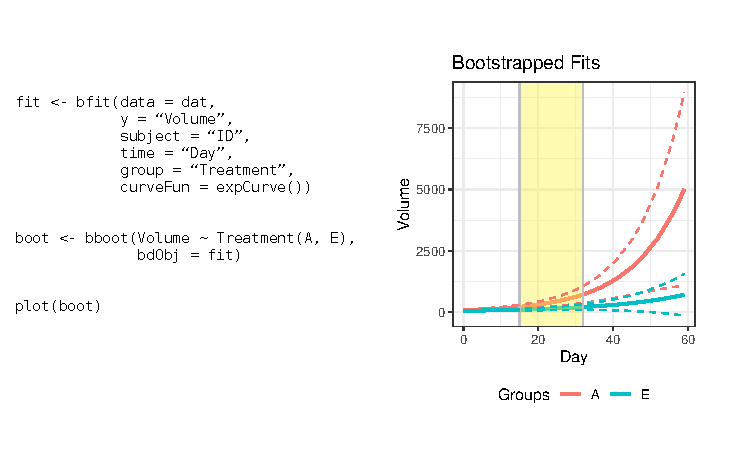
\includegraphics{bdots_examples.pdf}
\end{center}
\end{frame}




\begin{frame}{Concluding remarks}
What can we take away from this:
\begin{itemize}
\item VWP used to collect eye tracking data as proxy for word recognition
\item  Look onset method results in less bias in estimating generating curve
\item Software and methodology to investigate these
\end{itemize}
And where are we going from here?
\begin{itemize}
\item Oculomotor delay
\item Simulating eye tracking data (linking hypothesis)
\item Expanding domain of \texttt{bdots}
\end{itemize}
\end{frame}

%%------------------------------------END



\begin{frame}{References}\small
Magnuson, James S. \textbf{Fixations in the visual world paradigm: where, when, why?} 2019-09 \textit{Journal of Cultural Cognitive Science}, Vol. 3, No. 2 Springer  Science and Business Media LLC p. 113-139 \newline \\

McMurray, Bob \textbf{I'm not sure that curve means what you think it means: Towards a [more] realistic understanding of the role of eye-movement generation in the visual world paradigm} 2022 \textit{Psychonomic Bulletin \& Review} p 1-45 \newline \\

Oleson, Jacob J; Cavanaugh, Joseph E, McMurray, Bob; Brown, Grant \textbf{Detecting time-specific differences between temporal nonlinear curves: Analyzing data from the visual world paradigm} 2017 \textit{Statistical Methods in Medical Research}, Vol. 26, No. 6 p 2708-2725 \newline \\

Paul D. Allopenna, James S. Magnuson, Michael K. Tanenhaus
\textbf{Tracking the Time Course of Spoken Word Recognition Using Eye Movements: Evidence for Continuous Mapping Models} 1998 \textit{Journal of Memory and Language}, Vol. 38, Issue 4 p 419-439


\end{frame}



\end{document}